\chapter{Grafos direcionados}

Neste capítulo, nos concentramos em duas classes de grafos direcionados:
\begin{itemize}
\item \key{Grafos acíclicos}:
Não há ciclos no grafo,
portanto, não há caminho de nenhum nó para ele mesmo\footnote{Grafos direcionados acíclicos são às vezes chamados de DAGs.}.
\item \key{Grafos de sucessão}:
O grau de saída de cada nó é 1,
então cada nó tem um sucessor único.
\end{itemize}
Verifica-se que em ambos os casos,
podemos projetar algoritmos eficientes que são baseados
nas propriedades especiais dos grafos.

\section{Ordenação topológica}

\index{ordenação topológica}
\index{ciclo}

Uma \key{ordenação topológica} é uma ordenação
dos nós de um grafo direcionado
tal que se houver um caminho do nó $a$ para o nó $b$,
então o nó $a$ aparece antes do nó $b$ na ordenação.
Por exemplo, para o grafo
\begin{center}
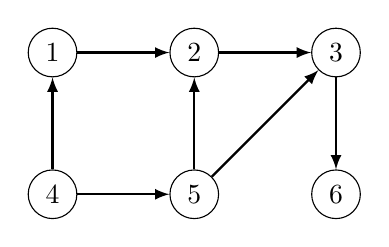
\begin{tikzpicture}[scale=0.9]
\node[draw, circle] (1) at (1,5) {$1$};
\node[draw, circle] (2) at (3,5) {$2$};
\node[draw, circle] (3) at (5,5) {$3$};
\node[draw, circle] (4) at (1,3) {$4$};
\node[draw, circle] (5) at (3,3) {$5$};
\node[draw, circle] (6) at (5,3) {$6$};

\path[draw,thick,->,>=latex] (1) -- (2);
\path[draw,thick,->,>=latex] (2) -- (3);
\path[draw,thick,->,>=latex] (4) -- (1);
\path[draw,thick,->,>=latex] (4) -- (5);
\path[draw,thick,->,>=latex] (5) -- (2);
\path[draw,thick,->,>=latex] (5) -- (3);
\path[draw,thick,->,>=latex] (3) -- (6);
\end{tikzpicture}
\end{center}
uma ordenação topológica é
$[4,1,5,2,3,6]$:
\begin{center}
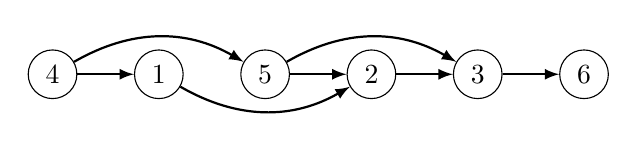
\begin{tikzpicture}[scale=0.9]
\node[draw, circle] (1) at (-6,0) {$1$};
\node[draw, circle] (2) at (-3,0) {$2$};
\node[draw, circle] (3) at (-1.5,0) {$3$};
\node[draw, circle] (4) at (-7.5,0) {$4$};
\node[draw, circle] (5) at (-4.5,0) {$5$};
\node[draw, circle] (6) at (-0,0) {$6$};

\path[draw,thick,->,>=latex] (1) edge [bend right=30] (2);
\path[draw,thick,->,>=latex] (2) -- (3);
\path[draw,thick,->,>=latex] (4) -- (1);
\path[draw,thick,->,>=latex] (4) edge [bend left=30] (5);
\path[draw,thick,->,>=latex] (5) -- (2);
\path[draw,thick,->,>=latex] (5) edge [bend left=30]  (3);
\path[draw,thick,->,>=latex] (3) -- (6);
\end{tikzpicture}
\end{center}

Um grafo acíclico sempre tem uma ordenação topológica.
No entanto, se o grafo contém um ciclo,
não é possível formar uma ordenação topológica,
porque nenhum nó do ciclo pode aparecer
antes dos outros nós do ciclo na ordenação.
Acontece que a busca em profundidade (DFS) pode ser usada
para verificar se um grafo direcionado contém um ciclo
e, se não contiver um ciclo, para construir uma ordenação topológica.

\subsubsection{Algoritmo}

A ideia é percorrer os nós do grafo
e sempre iniciar uma busca em profundidade no nó atual
se ele ainda não tiver sido processado.
Durante as buscas, os nós têm três estados possíveis:

\begin{itemize}
\item estado 0: o nó não foi processado (branco)
\item estado 1: o nó está sendo processado (cinza claro)
\item estado 2: o nó foi processado (cinza escuro)
\end{itemize}

Inicialmente, o estado de cada nó é 0.
Quando uma busca chega a um nó pela primeira vez,
seu estado muda para 1.
Finalmente, depois que todos os sucessores do nó tiverem
sido processados, seu estado muda para 2.

Se o grafo contém um ciclo, descobriremos isso
durante a busca, porque mais cedo ou mais tarde
chegaremos a um nó cujo estado é 1.
Nesse caso, não é possível construir uma ordenação topológica.

Se o grafo não contiver um ciclo, podemos construir
uma ordenação topológica adicionando cada nó a uma lista quando o estado do nó se tornar 2.
Esta lista em ordem inversa é uma ordenação topológica.

\subsubsection{Exemplo 1}

No grafo de exemplo, a busca prossegue primeiro
do nó 1 ao nó 6:

\begin{center}
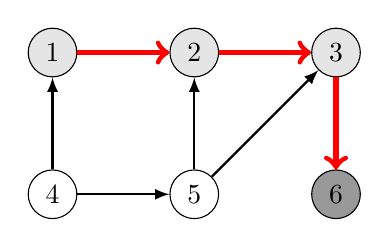
\begin{tikzpicture}[scale=0.9]
\node[draw, circle,fill=gray!20] (1) at (1,5) {$1$};
\node[draw, circle,fill=gray!20] (2) at (3,5) {$2$};
\node[draw, circle,fill=gray!20] (3) at (5,5) {$3$};
\node[draw, circle] (4) at (1,3) {$4$};
\node[draw, circle] (5) at (3,3) {$5$};
\node[draw, circle,fill=gray!80] (6) at (5,3) {$6$};

\path[draw,thick,->,>=latex] (4) -- (1);
\path[draw,thick,->,>=latex] (4) -- (5);
\path[draw,thick,->,>=latex] (5) -- (2);
\path[draw,thick,->,>=latex] (5) -- (3);
%\path[draw,thick,->,>=latex] (3) -- (6);

\path[draw=red,thick,->,line width=2pt] (1) -- (2);
\path[draw=red,thick,->,line width=2pt] (2) -- (3);
\path[draw=red,thick,->,line width=2pt] (3) -- (6);
\end{tikzpicture}
\end{center}

Agora, o nó 6 foi processado e adicionado à lista.
Depois disso, os nós 3, 2 e 1 também são adicionados à lista:

\begin{center}
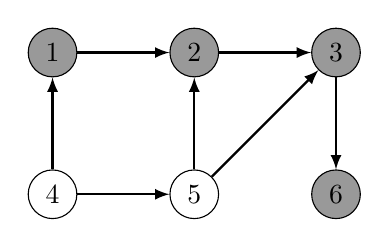
\begin{tikzpicture}[scale=0.9]
\node[draw, circle,fill=gray!80] (1) at (1,5) {$1$};
\node[draw, circle,fill=gray!80] (2) at (3,5) {$2$};
\node[draw, circle,fill=gray!80] (3) at (5,5) {$3$};
\node[draw, circle] (4) at (1,3) {$4$};
\node[draw, circle] (5) at (3,3) {$5$};
\node[draw, circle,fill=gray!80] (6) at (5,3) {$6$};

\path[draw,thick,->,>=latex] (1) -- (2);
\path[draw,thick,->,>=latex] (2) -- (3);
\path[draw,thick,->,>=latex] (4) -- (1);
\path[draw,thick,->,>=latex] (4) -- (5);
\path[draw,thick,->,>=latex] (5) -- (2);
\path[draw,thick,->,>=latex] (5) -- (3);
\path[draw,thick,->,>=latex] (3) -- (6);
\end{tikzpicture}
\end{center}

Neste ponto, a lista é $[6,3,2,1]$.
A próxima pesquisa começa no nó 4:

\begin{center}
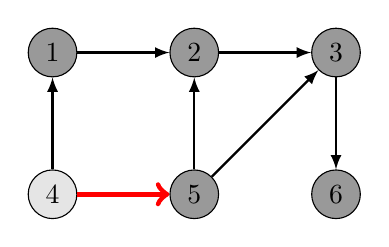
\begin{tikzpicture}[scale=0.9]
\node[draw, circle,fill=gray!80] (1) at (1,5) {$1$};
\node[draw, circle,fill=gray!80] (2) at (3,5) {$2$};
\node[draw, circle,fill=gray!80] (3) at (5,5) {$3$};
\node[draw, circle,fill=gray!20] (4) at (1,3) {$4$};
\node[draw, circle,fill=gray!80] (5) at (3,3) {$5$};
\node[draw, circle,fill=gray!80] (6) at (5,3) {$6$};

\path[draw,thick,->,>=latex] (1) -- (2);
\path[draw,thick,->,>=latex] (2) -- (3);
\path[draw,thick,->,>=latex] (4) -- (1);
%\path[draw,thick,->,>=latex] (4) -- (5);
\path[draw,thick,->,>=latex] (5) -- (2);
\path[draw,thick,->,>=latex] (5) -- (3);
\path[draw,thick,->,>=latex] (3) -- (6);

\path[draw=red,thick,->,line width=2pt] (4) -- (5);
\end{tikzpicture}
\end{center}

Assim, a lista final é $[6,3,2,1,5,4]$.
Processamos todos os nós, então uma ordenação topológica foi
encontrada.
A ordenação topológica é a lista inversa
$[4,5,1,2,3,6]$:

\begin{center}
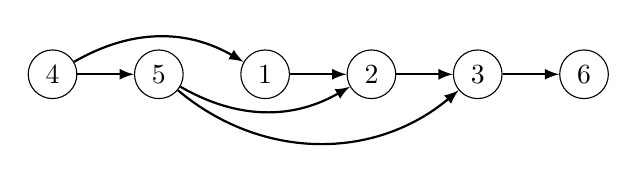
\begin{tikzpicture}[scale=0.9]
\node[draw, circle] (1) at (3,0) {$1$};
\node[draw, circle] (2) at (4.5,0) {$2$};
\node[draw, circle] (3) at (6,0) {$3$};
\node[draw, circle] (4) at (0,0) {$4$};
\node[draw, circle] (5) at (1.5,0) {$5$};
\node[draw, circle] (6) at (7.5,0) {$6$};

\path[draw,thick,->,>=latex] (1) -- (2);
\path[draw,thick,->,>=latex] (2) -- (3);
\path[draw,thick,->,>=latex] (4) edge [bend left=30] (1);
\path[draw,thick,->,>=latex] (4) -- (5);
\path[draw,thick,->,>=latex] (5) edge [bend right=30] (2);
\path[draw,thick,->,>=latex] (5) edge [bend right=40] (3);
\path[draw,thick,->,>=latex] (3) -- (6);
\end{tikzpicture}
\end{center}

Observe que uma ordenação topológica não é única,
e pode haver várias ordenações topológicas para um grafo.

\subsubsection{Exemplo 2}

Vamos agora considerar um grafo para o qual nós
não podemos construir uma ordenação topológica,
porque o grafo contém um ciclo:

\begin{center}
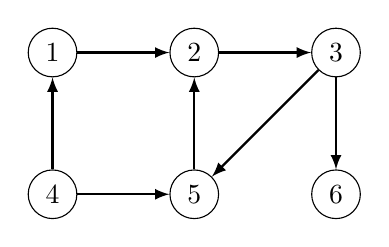
\begin{tikzpicture}[scale=0.9]
\node[draw, circle] (1) at (1,5) {$1$};
\node[draw, circle] (2) at (3,5) {$2$};
\node[draw, circle] (3) at (5,5) {$3$};
\node[draw, circle] (4) at (1,3) {$4$};
\node[draw, circle] (5) at (3,3) {$5$};
\node[draw, circle] (6) at (5,3) {$6$};

\path[draw,thick,->,>=latex] (1) -- (2);
\path[draw,thick,->,>=latex] (2) -- (3);
\path[draw,thick,->,>=latex] (4) -- (1);
\path[draw,thick,->,>=latex] (4) -- (5);
\path[draw,thick,->,>=latex] (5) -- (2);
\path[draw,thick,->,>=latex] (3) -- (5);
\path[draw,thick,->,>=latex] (3) -- (6);
\end{tikzpicture}
\end{center}
A pesquisa prossegue da seguinte forma:
\begin{center}
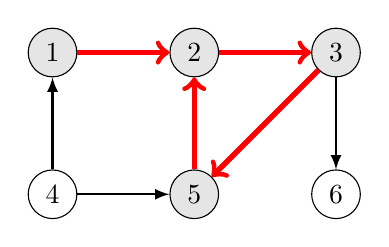
\begin{tikzpicture}[scale=0.9]
\node[draw, circle,fill=gray!20] (1) at (1,5) {$1$};
\node[draw, circle,fill=gray!20] (2) at (3,5) {$2$};
\node[draw, circle,fill=gray!20] (3) at (5,5) {$3$};
\node[draw, circle] (4) at (1,3) {$4$};
\node[draw, circle,fill=gray!20] (5) at (3,3) {$5$};
\node[draw, circle] (6) at (5,3) {$6$};

\path[draw,thick,->,>=latex] (4) -- (1);
\path[draw,thick,->,>=latex] (4) -- (5);
\path[draw,thick,->,>=latex] (3) -- (6);

\path[draw=red,thick,->,line width=2pt] (1) -- (2);
\path[draw=red,thick,->,line width=2pt] (2) -- (3);
\path[draw=red,thick,->,line width=2pt] (3) -- (5);
\path[draw=red,thick,->,line width=2pt] (5) -- (2);
\end{tikzpicture}
\end{center}
A busca chega ao nó 2, cujo estado é 1,
o que significa que o grafo contém um ciclo.
Neste exemplo, há um ciclo
$2 \rightarrow 3 \rightarrow 5 \rightarrow 2$.

\section{Programação dinâmica}

Se um grafo direcionado for acíclico,
a programação dinâmica pode ser aplicada a ele.
Por exemplo, podemos resolver eficientemente os seguintes
problemas relativos a caminhos de um nó inicial
para um nó final:

\begin{itemize}
\item quantos caminhos diferentes existem?
\item qual é o caminho mais curto/longo?
\item qual é o número mínimo/máximo de arestas em um caminho?
\item quais nós certamente aparecem em qualquer caminho?
\end{itemize}

\subsubsection{Contando o número de caminhos}

Como exemplo, vamos calcular o número de caminhos
do nó 1 ao nó 6 no seguinte grafo:

\begin{center}
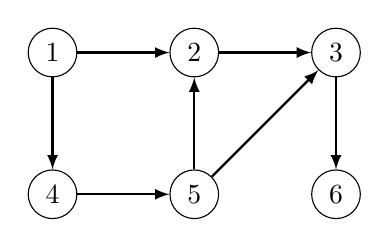
\begin{tikzpicture}[scale=0.9]
\node[draw, circle] (1) at (1,5) {$1$};
\node[draw, circle] (2) at (3,5) {$2$};
\node[draw, circle] (3) at (5,5) {$3$};
\node[draw, circle] (4) at (1,3) {$4$};
\node[draw, circle] (5) at (3,3) {$5$};
\node[draw, circle] (6) at (5,3) {$6$};

\path[draw,thick,->,>=latex] (1) -- (2);
\path[draw,thick,->,>=latex] (2) -- (3);
\path[draw,thick,->,>=latex] (1) -- (4);
\path[draw,thick,->,>=latex] (4) -- (5);
\path[draw,thick,->,>=latex] (5) -- (2);
\path[draw,thick,->,>=latex] (5) -- (3);
\path[draw,thick,->,>=latex] (3) -- (6);
\end{tikzpicture}
\end{center}
Existem no total três desses caminhos:
\begin{itemize}
\item $1 \rightarrow 2 \rightarrow 3 \rightarrow 6$
\item $1 \rightarrow 4 \rightarrow 5 \rightarrow 2 \rightarrow 3 \rightarrow 6$
\item $1 \rightarrow 4 \rightarrow 5 \rightarrow 3 \rightarrow 6$
\end{itemize}

Seja $\texttt{paths}(x)$ o número de caminhos de
nó 1 ao nó $x$.
Como caso base, $\texttt{paths}(1)=1$.
Então, para calcular outros valores de $\texttt{paths}(x)$,
podemos usar a recursão
\[\texttt{paths}(x) = \texttt{paths}(a_1)+\texttt{paths}(a_2)+\cdots+\texttt{paths}(a_k)\]
onde $a_1,a_2,\ldots,a_k$ são os nós dos quais
há uma aresta para $x$.
Como o grafo é acíclico, os valores de $\texttt{paths}(x)$
pode ser calculado na ordem de uma ordenação topológica.
Uma ordenação topológica para o grafo acima é a seguinte:
\begin{center}
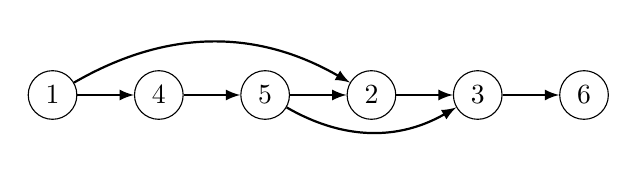
\begin{tikzpicture}[scale=0.9]
\node[draw, circle] (1) at (0,0) {$1$};
\node[draw, circle] (2) at (4.5,0) {$2$};
\node[draw, circle] (3) at (6,0) {$3$};
\node[draw, circle] (4) at (1.5,0) {$4$};
\node[draw, circle] (5) at (3,0) {$5$};
\node[draw, circle] (6) at (7.5,0) {$6$};

\path[draw,thick,->,>=latex] (1) edge [bend left=30] (2);
\path[draw,thick,->,>=latex] (2) -- (3);
\path[draw,thick,->,>=latex] (1) -- (4);
\path[draw,thick,->,>=latex] (4) -- (5);
\path[draw,thick,->,>=latex] (5) -- (2);
\path[draw,thick,->,>=latex] (5) edge [bend right=30] (3);
\path[draw,thick,->,>=latex] (3) -- (6);
\end{tikzpicture}
\end{center}
Portanto, os números de caminhos são os seguintes:
\begin{center}
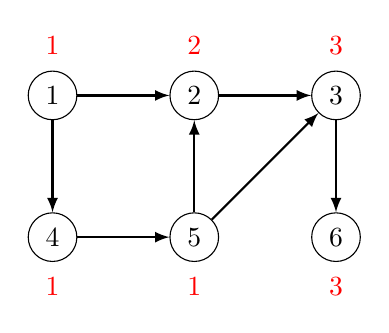
\begin{tikzpicture}[scale=0.9]
\node[draw, circle] (1) at (1,5) {$1$};
\node[draw, circle] (2) at (3,5) {$2$};
\node[draw, circle] (3) at (5,5) {$3$};
\node[draw, circle] (4) at (1,3) {$4$};
\node[draw, circle] (5) at (3,3) {$5$};
\node[draw, circle] (6) at (5,3) {$6$};

\path[draw,thick,->,>=latex] (1) -- (2);
\path[draw,thick,->,>=latex] (2) -- (3);
\path[draw,thick,->,>=latex] (1) -- (4);
\path[draw,thick,->,>=latex] (4) -- (5);
\path[draw,thick,->,>=latex] (5) -- (2);
\path[draw,thick,->,>=latex] (5) -- (3);
\path[draw,thick,->,>=latex] (3) -- (6);

\node[color=red] at (1,2.3) {$1$};
\node[color=red] at (3,2.3) {$1$};
\node[color=red] at (5,2.3) {$3$};
\node[color=red] at (1,5.7) {$1$};
\node[color=red] at (3,5.7) {$2$};
\node[color=red] at (5,5.7) {$3$};
\end{tikzpicture}
\end{center}

Por exemplo, para calcular o valor de $\texttt{paths}(3)$,
podemos usar a fórmula $\texttt{paths}(2)+\texttt{paths}(5)$,
porque existem arestas dos nós 2 e 5
para o nó 3.
Como $\texttt{paths}(2)=2$ e $\texttt{paths}(5)=1$, concluímos que $\texttt{paths}(3)=3$.

\subsubsection{Estendendo o algoritmo de Dijkstra}

\index{algoritmo de Dijkstra}

Um subproduto do algoritmo de Dijkstra é um grafo direcionado e acíclico
que indica para cada nó do grafo original
as maneiras possíveis de alcançar o nó usando um caminho mais curto
do nó inicial.
A programação dinâmica pode ser aplicada a esse grafo.
Por exemplo, no grafo
\begin{center}
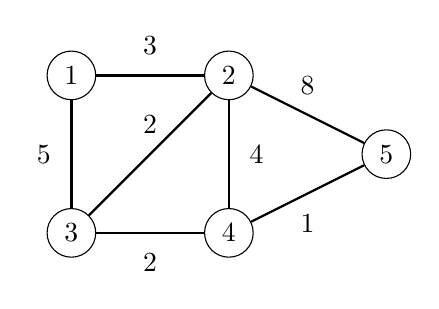
\begin{tikzpicture}
\node[draw, circle] (1) at (0,0) {$1$};
\node[draw, circle] (2) at (2,0) {$2$};
\node[draw, circle] (3) at (0,-2) {$3$};
\node[draw, circle] (4) at (2,-2) {$4$};
\node[draw, circle] (5) at (4,-1) {$5$};

\path[draw,thick,-] (1) -- node[font=\small,label=above:3] {} (2);
\path[draw,thick,-] (1) -- node[font=\small,label=left:5] {} (3);
\path[draw,thick,-] (2) -- node[font=\small,label=right:4] {} (4);
\path[draw,thick,-] (2) -- node[font=\small,label=above:8] {} (5);
\path[draw,thick,-] (3) -- node[font=\small,label=below:2] {} (4);
\path[draw,thick,-] (4) -- node[font=\small,label=below:1] {} (5);
\path[draw,thick,-] (2) -- node[font=\small,label=above:2] {} (3);
\end{tikzpicture}
\end{center}
os caminhos mais curtos do nó 1 podem usar as seguintes arestas:
\begin{center}
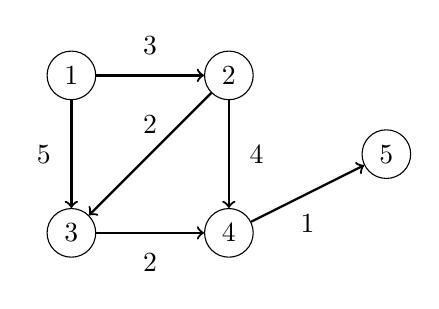
\begin{tikzpicture}
\node[draw, circle] (1) at (0,0) {$1$};
\node[draw, circle] (2) at (2,0) {$2$};
\node[draw, circle] (3) at (0,-2) {$3$};
\node[draw, circle] (4) at (2,-2) {$4$};
\node[draw, circle] (5) at (4,-1) {$5$};

\path[draw,thick,->] (1) -- node[font=\small,label=above:3] {} (2);
\path[draw,thick,->] (1) -- node[font=\small,label=left:5] {} (3);
\path[draw,thick,->] (2) -- node[font=\small,label=right:4] {} (4);
\path[draw,thick,->] (3) -- node[font=\small,label=below:2] {} (4);
\path[draw,thick,->] (4) -- node[font=\small,label=below:1] {} (5);
\path[draw,thick,->] (2) -- node[font=\small,label=above:2] {} (3);
\end{tikzpicture}
\end{center}

Agora podemos, por exemplo, calcular o número de
caminhos mais curtos do nó 1 ao nó 5
usando programação dinâmica:
\begin{center}
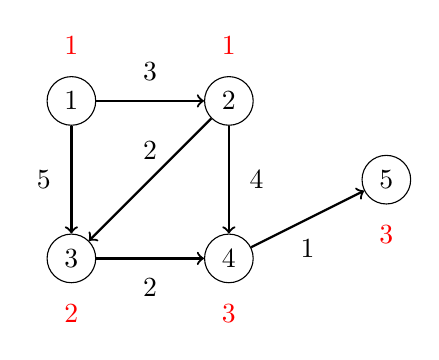
\begin{tikzpicture}
\node[draw, circle] (1) at (0,0) {$1$};
\node[draw, circle] (2) at (2,0) {$2$};
\node[draw, circle] (3) at (0,-2) {$3$};
\node[draw, circle] (4) at (2,-2) {$4$};
\node[draw, circle] (5) at (4,-1) {$5$};

\path[draw,thick,->] (1) -- node[font=\small,label=above:3] {} (2);
\path[draw,thick,->] (1) -- node[font=\small,label=left:5] {} (3);
\path[draw,thick,->] (2) -- node[font=\small,label=right:4] {} (4);
\path[draw,thick,->] (3) -- node[font=\small,label=below:2] {} (4);
\path[draw,thick,->] (4) -- node[font=\small,label=below:1] {} (5);
\path[draw,thick,->] (2) -- node[font=\small,label=above:2] {} (3);

\node[color=red] at (0,0.7) {$1$};
\node[color=red] at (2,0.7) {$1$};
\node[color=red] at (0,-2.7) {$2$};
\node[color=red] at (2,-2.7) {$3$};
\node[color=red] at (4,-1.7) {$3$};
\end{tikzpicture}
\end{center}

\subsubsection{Representando problemas como grafos}

Na verdade, qualquer problema de programação dinâmica
pode ser representado como um grafo direcionado e acíclico.
Em tal grafo, cada nó corresponde a um estado de programação dinâmica
e as arestas indicam como os estados dependem uns dos outros.

Como exemplo, considere o problema
de formar uma soma de dinheiro $n$
usando moedas
$\{c_1,c_2,\ldots,c_k\}$.
Neste problema, podemos construir um grafo onde
cada nó corresponde a uma soma de dinheiro,
e as arestas mostram como as moedas podem ser escolhidas.
Por exemplo, para moedas $\{1,3,4\}$ e $n=6$,
o grafo é o seguinte:
\begin{center}
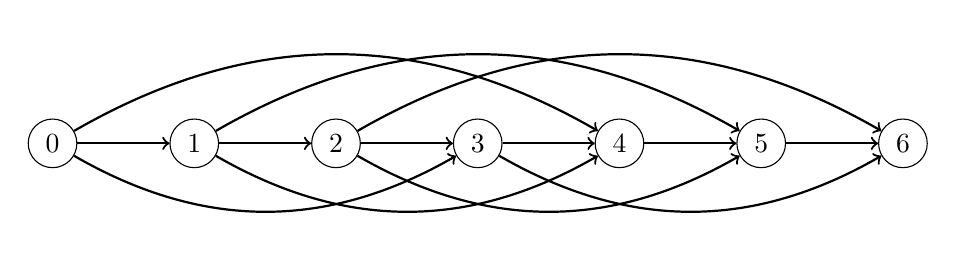
\begin{tikzpicture}[scale=0.9]
\node[draw, circle] (0) at (0,0) {$0$};
\node[draw, circle] (1) at (2,0) {$1$};
\node[draw, circle] (2) at (4,0) {$2$};
\node[draw, circle] (3) at (6,0) {$3$};
\node[draw, circle] (4) at (8,0) {$4$};
\node[draw, circle] (5) at (10,0) {$5$};
\node[draw, circle] (6) at (12,0) {$6$};

\path[draw,thick,->] (0) -- (1);
\path[draw,thick,->] (1) -- (2);
\path[draw,thick,->] (2) -- (3);
\path[draw,thick,->] (3) -- (4);
\path[draw,thick,->] (4) -- (5);
\path[draw,thick,->] (5) -- (6);

\path[draw,thick,->] (0) edge [bend right=30] (3);
\path[draw,thick,->] (1) edge [bend right=30] (4);
\path[draw,thick,->] (2) edge [bend right=30] (5);
\path[draw,thick,->] (3) edge [bend right=30] (6);

\path[draw,thick,->] (0) edge [bend left=30] (4);
\path[draw,thick,->] (1) edge [bend left=30] (5);
\path[draw,thick,->] (2) edge [bend left=30] (6);
\end{tikzpicture}
\end{center}

Usando esta representação,
o caminho mais curto do nó 0 ao nó $n$
corresponde a uma solução com o número mínimo de moedas,
e o número total de caminhos do nó 0 ao nó $n$
é igual ao número total de soluções.

\section{Caminhos sucessores}

\index{grafo de sucessores}
\index{grafo funcional}

No restante deste capítulo,
vamos nos concentrar em \key{grafos de sucessores}.
Nesses grafos,
o grau de saída de cada nó é 1, ou seja,
exatamente uma aresta começa em cada nó.
Um grafo de sucessores consiste em um ou mais
componentes, cada um contendo
um ciclo e alguns caminhos que levam a ele.

Os grafos de sucessores são às vezes chamados
de \key{grafos funcionais}.
A razão para isso é que qualquer grafo de sucessores
corresponde a uma função que define
as arestas do grafo.
O parâmetro para a função é um nó do grafo,
e a função fornece o sucessor desse nó.

Por exemplo, a função
\begin{center}
\begin{tabular}{r|rrrrrrrrr}
$x$ & 1 & 2 & 3 & 4 & 5 & 6 & 7 & 8 & 9 \\
\hline
$\texttt{succ}(x)$ & 3 & 5 & 7 & 6 & 2 & 2 & 1 & 6 & 3 \\
\end{tabular}
\end{center}
define o seguinte grafo:
\begin{center}
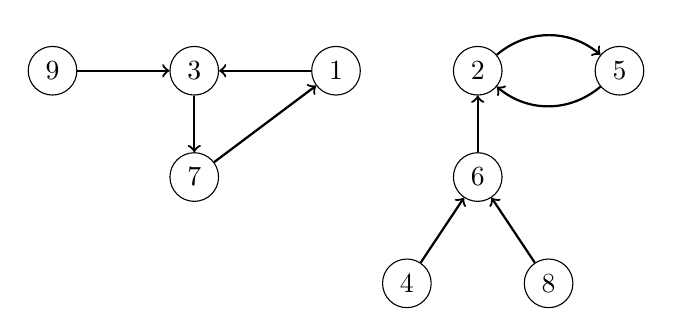
\begin{tikzpicture}[scale=0.9]
\node[draw, circle] (1) at (0,0) {$1$};
\node[draw, circle] (2) at (2,0) {$2$};
\node[draw, circle] (3) at (-2,0) {$3$};
\node[draw, circle] (4) at (1,-3) {$4$};
\node[draw, circle] (5) at (4,0) {$5$};
\node[draw, circle] (6) at (2,-1.5) {$6$};
\node[draw, circle] (7) at (-2,-1.5) {$7$};
\node[draw, circle] (8) at (3,-3) {$8$};
\node[draw, circle] (9) at (-4,0) {$9$};

\path[draw,thick,->] (1) -- (3);
\path[draw,thick,->] (2)  edge [bend left=40] (5);
\path[draw,thick,->] (3) -- (7);
\path[draw,thick,->] (4) -- (6);
\path[draw,thick,->] (5)  edge [bend left=40] (2);
\path[draw,thick,->] (6) -- (2);
\path[draw,thick,->] (7) -- (1);
\path[draw,thick,->] (8) -- (6);
\path[draw,thick,->] (9) -- (3);
\end{tikzpicture}
\end{center}

Como cada nó de um grafo de sucessores tem um
único sucessor, também podemos definir uma função $\texttt{succ}(x,k)$
que retorna o nó ao qual chegaremos se
começarmos no nó $x$ e andarmos $k$ passos para frente.
Por exemplo, no grafo acima $\texttt{succ}(4,6)=2$,
porque chegaremos ao nó 2 caminhando 6 passos a partir do nó 4:

\begin{center}
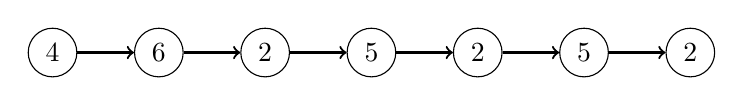
\begin{tikzpicture}[scale=0.9]
\node[draw, circle] (1) at (0,0) {$4$};
\node[draw, circle] (2) at (1.5,0) {$6$};
\node[draw, circle] (3) at (3,0) {$2$};
\node[draw, circle] (4) at (4.5,0) {$5$};
\node[draw, circle] (5) at (6,0) {$2$};
\node[draw, circle] (6) at (7.5,0) {$5$};
\node[draw, circle] (7) at (9,0) {$2$};

\path[draw,thick,->] (1) -- (2);
\path[draw,thick,->] (2) -- (3);
\path[draw,thick,->] (3) -- (4);
\path[draw,thick,->] (4) -- (5);
\path[draw,thick,->] (5) -- (6);
\path[draw,thick,->] (6) -- (7);
\end{tikzpicture}
\end{center}

Uma maneira direta de calcular um valor de $\texttt{succ}(x,k)$
é começar no nó $x$ e andar $k$ passos para frente, o que leva um tempo $O(k)$.
No entanto, usando pré-processamento, qualquer valor de $\texttt{succ}(x,k)$
pode ser calculado em apenas um tempo $O(\log k)$.

A ideia é pré-calcular todos os valores de $\texttt{succ}(x,k)$ onde
$k$ é uma potência de dois e no máximo $u$, onde $u$ é
o número máximo de passos que jamais daremos.
Isso pode ser feito de forma eficiente, pois
podemos usar a seguinte recursão:

\begin{equation*}
    \texttt{succ}(x,k) = \begin{cases}
               \texttt{succ}(x)              & k = 1\\
               \texttt{succ}(\texttt{succ}(x,k/2),k/2)   & k > 1\\
           \end{cases}
\end{equation*}

Pré-calcular os valores leva um tempo $O(n \log u)$,
porque $O(\log u)$ valores são calculados para cada nó.
No grafo acima, os primeiros valores são os seguintes:

\begin{center}
\begin{tabular}{r|rrrrrrrrr}
$x$ & 1 & 2 & 3 & 4 & 5 & 6 & 7 & 8 & 9 \\
\hline
$\texttt{succ}(x,1)$ & 3 & 5 & 7 & 6 & 2 & 2 & 1 & 6 & 3 \\
$\texttt{succ}(x,2)$ & 7 & 2 & 1 & 2 & 5 & 5 & 3 & 2 & 7 \\
$\texttt{succ}(x,4)$ & 3 & 2 & 7 & 2 & 5 & 5 & 1 & 2 & 3 \\
$\texttt{succ}(x,8)$ & 7 & 2 & 1 & 2 & 5 & 5 & 3 & 2 & 7 \\
$\cdots$ \\
\end{tabular}
\end{center}

Depois disso, qualquer valor de $\texttt{succ}(x,k)$ pode ser calculado
representando o número de passos $k$ como uma soma de potências de dois.
Por exemplo, se quisermos calcular o valor de $\texttt{succ}(x,11)$,
primeiro formamos a representação $11=8+2+1$.
Usando isso,
\[\texttt{succ}(x,11)=\texttt{succ}(\texttt{succ}(\texttt{succ}(x,8),2),1).\]
Por exemplo, no grafo anterior
\[\texttt{succ}(4,11)=\texttt{succ}(\texttt{succ}(\texttt{succ}(4,8),2),1)=5.\]

Essa representação sempre consiste em
$O(\log k)$ partes, então calcular um valor de $\texttt{succ}(x,k)$
leva um tempo $O(\log k)$.

\section{Detecção de ciclo}

\index{ciclo}
\index{detecção de ciclo}

Considere um grafo de sucessores que contém apenas
um caminho que termina em um ciclo.
Podemos fazer as seguintes perguntas:
se começarmos nossa caminhada no nó inicial,
qual é o primeiro nó no ciclo
e quantos nós o ciclo contém?

Por exemplo, no grafo

\begin{center}
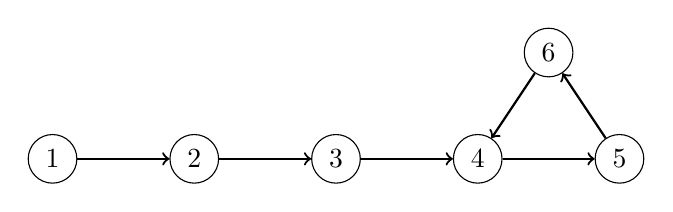
\begin{tikzpicture}[scale=0.9]
\node[draw, circle] (5) at (0,0) {$5$};
\node[draw, circle] (4) at (-2,0) {$4$};
\node[draw, circle] (6) at (-1,1.5) {$6$};
\node[draw, circle] (3) at (-4,0) {$3$};
\node[draw, circle] (2) at (-6,0) {$2$};
\node[draw, circle] (1) at (-8,0) {$1$};

\path[draw,thick,->] (1) -- (2);
\path[draw,thick,->] (2) -- (3);
\path[draw,thick,->] (3) -- (4);
\path[draw,thick,->] (4) -- (5);
\path[draw,thick,->] (5) -- (6);
\path[draw,thick,->] (6) -- (4);
\end{tikzpicture}
\end{center}
começamos nossa caminhada no nó 1,
o primeiro nó que pertence ao ciclo é o nó 4, e o ciclo consiste
em três nós (4, 5 e 6).

Uma maneira simples de detectar o ciclo é caminhar no
grafo e manter o controle de
todos os nós que foram visitados. Uma vez que um nó é visitado
pela segunda vez, podemos concluir
que o nó é o primeiro nó no ciclo.
Este método funciona em tempo $O(n)$ e também usa
memória $O(n)$.

No entanto, existem algoritmos melhores para detecção de ciclo.
A complexidade de tempo de tais algoritmos ainda é $O(n)$,
mas eles usam apenas memória $O(1)$.
Esta é uma melhoria importante se $n$ for grande.
A seguir, discutiremos o algoritmo de Floyd que
alcança essas propriedades.

\subsubsection{Algoritmo de Floyd}

\index{Algoritmo de Floyd}

O \key{algoritmo de Floyd}\footnote{A ideia do algoritmo é mencionada em \cite{knu982}
e atribuída a R. W. Floyd; no entanto, não se sabe se Floyd realmente
descobriu o algoritmo.} caminha para frente
no grafo usando dois ponteiros $a$ e $b$.
Ambos os ponteiros começam em um nó $x$ que
é o nó inicial do grafo.
Então, a cada turno, o ponteiro $a$ caminha
um passo para frente e o ponteiro $b$
caminha dois passos para frente.
O processo continua até
que os ponteiros se encontrem:
\begin{lstlisting}
a = succ(x);
b = succ(succ(x));
while (a != b) {
    a = succ(a);
    b = succ(succ(b));
}
\end{lstlisting}

Neste ponto, o ponteiro $a$ caminhou $k$ passos
e o ponteiro $b$ caminhou $2k$ passos,
então o comprimento do ciclo divide $k$.
Assim, o primeiro nó que pertence ao ciclo
pode ser encontrado movendo o ponteiro $a$ para o nó $x$
e avançando os ponteiros
passo a passo até que se encontrem novamente.
\begin{lstlisting}
a = x;
while (a != b) {
    a = succ(a);
    b = succ(b);
}
primeiro = a;
\end{lstlisting}

Depois disso, o comprimento do ciclo
pode ser calculado da seguinte forma:
\begin{lstlisting}
b = succ(a);
comprimento = 1;
while (a != b) {
    b = succ(b);
    comprimento++;
}
\end{lstlisting}
